\documentclass[tikz]{standalone}
\usetikzlibrary{calc}
\usepackage{pgfplots}
\usepgfplotslibrary{polar}
\pgfplotsset{compat=1.11}

\begin{document}

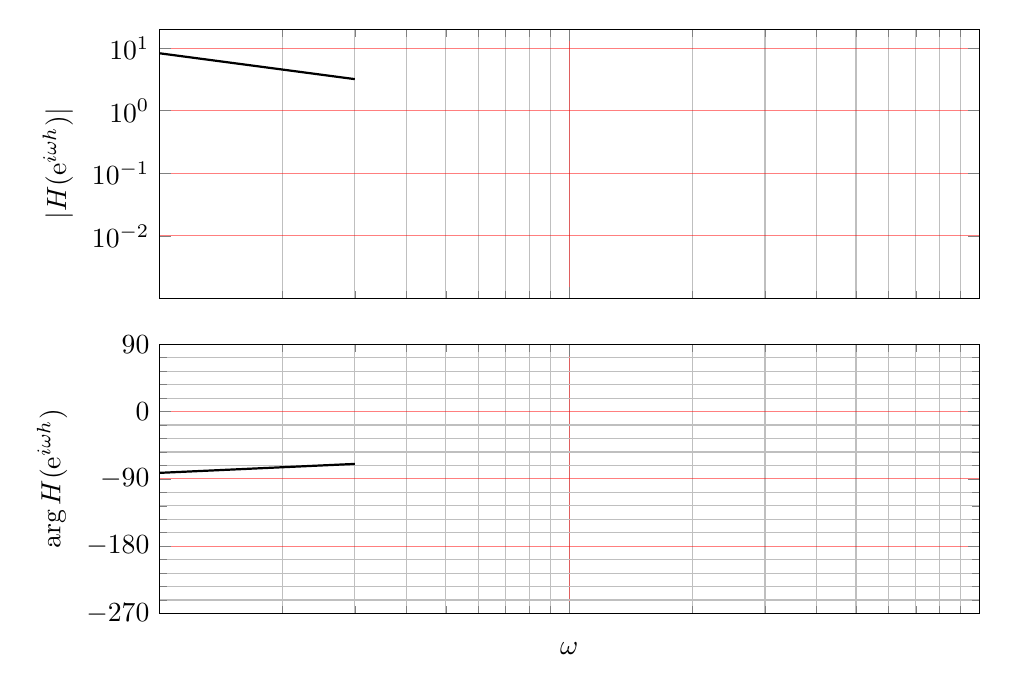
\begin{tikzpicture}
  \begin{loglogaxis} [
      width=12cm,
      height=5cm,
      ylabel=$|H(\mathrm{e}^{i\omega h})|$,
      xticklabels=\empty,
      ytick={10, 1, 0.1, 0.01},
      ymax=20,
      ymin=0.001,
      xmin=0.1,
      xmax=10,
      grid=both,
      minor y tick num=9,
%      extra y ticks={.5}, % how to convert to fixed point tick label ?
%      extra y tick style={log identify minor tick positions=true},
      every major grid/.style={red, opacity=0.5},
  ]


    \addplot [thick, black, no marks] coordinates {(0.1, 8.3) (0.3, 3.2)};

  \end{loglogaxis}
  \begin{semilogxaxis} [
      xlabel=$\omega$,
      ylabel=$\arg H(\mathrm{e}^{i\omega h})$,
      yshift = -4cm, 
      width=12cm,
      height=5cm,
      grid=both,
      ytick={90, 0, -90, -180, -270},
      ymax= 90,
      ymin=-270,
      xmin=0.1,
      xmax=10,
      minor y tick num=4,
      every major grid/.style={red, opacity=0.5},
      xticklabels=\empty,
  ]
    \addplot [thick, black, no marks] coordinates {(0.1, -82) (0.3, -70)};

  \end{semilogxaxis}
\end{tikzpicture}

\end{document}
